\section{Requisitos da Experiência Meta 5}
A elaboração da Meta 4 consistia em adicionar um servidor Proxy ao Cluster. Neste momento com a Meta 4 concluída verificamos que existe um ponto critico chamado de \ac{SPOF}. Este \ac{SPOF} não é nada mais do que existir apenas um servidor Proxy o que quer dizer que se acontecer algum problema no servidor Proxy o sistema fica comprometido. 

A meta 5 consiste em eliminar o \ac{SPOF} criado na meta 4 e para isso vamos adicionar mais um servidor Proxy e instalar e proceder a devida configuração do Keepalived.


\hfill \break
\indent Endereçamento Meta 5:
\begin{table}[h]
\begin{center}
\begin{tabular}{||c c||} 
 \hline
 Nome & IP\\ [0.5ex] 
 \hline\hline
 Node 1 & 192.168.1.118\\ 
 \hline
 Node 2 & 192.168.1.119\\
 \hline
 Node 3 & 192.168.1.120\\
 \hline
 Sysbench & 192.168.1.121\\
 \hline
 Proxy & 192.168.1.122\\
 \hline
 Proxy1 & 192.168.1.125\\
 \hline
\end{tabular}
\caption{Tabela endereçamento IP Meta 5}
\end{center}
\end{table}

\newpage
\section{Segundo Proxy}
Para adicionar um segundo Proxy comecei por criar mais uma \ac{VM} (proxy1) com as mesmas configurações já mencionadas na meta 4.

Antes de proceder á instalação do Keepalived foi preciso repetir o processo de criação do ProxySQL neste Proxy1. Para isso bastou seguir os passos do Capitulo 9.9 Proxy.
No final verifiquei o \textit{status} do ProxySQL:

\begin{figure}[H]
\center
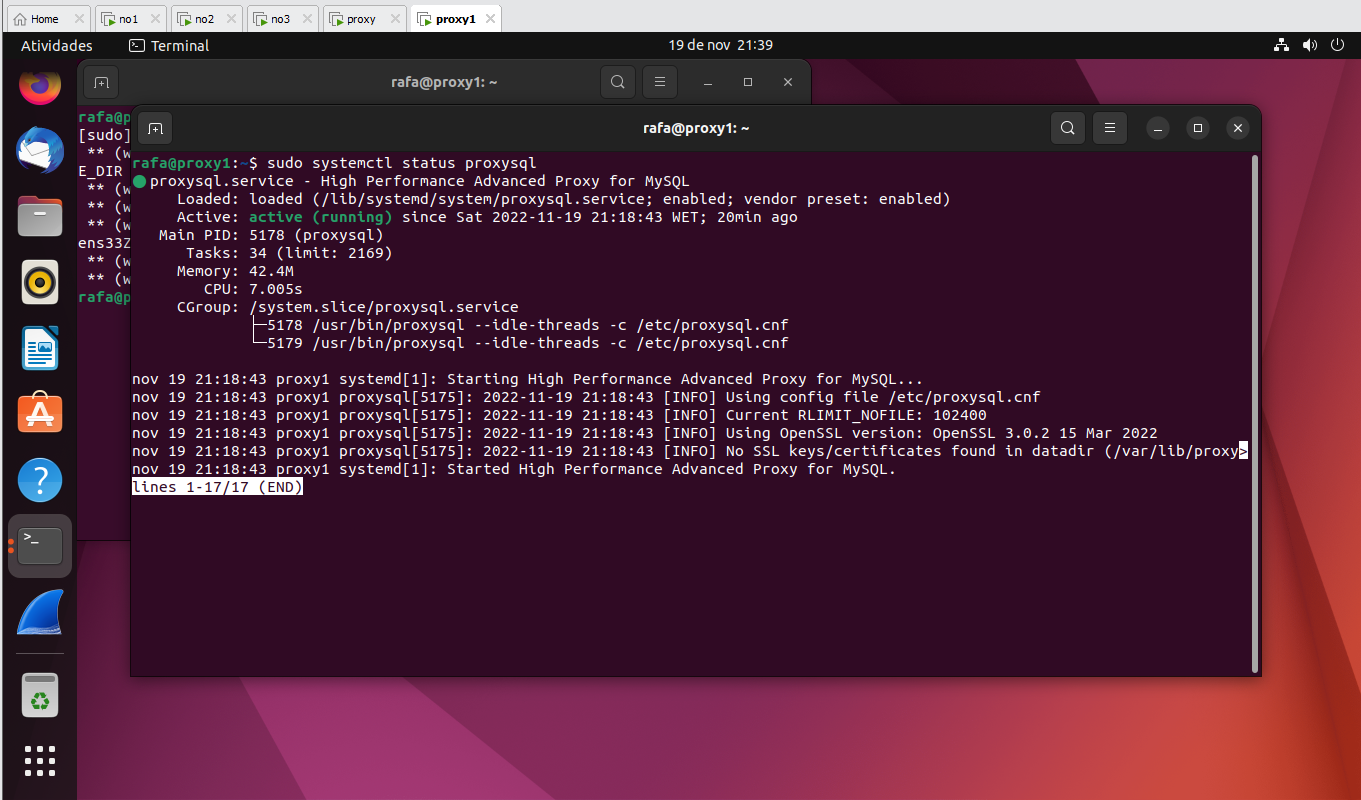
\includegraphics[width=13cm]{status_proxy1.png}
\caption{Status ProxySQL Proxy1}
\end{figure}

Com a autenticação do utilizador MySQL criado, verifiquei também se neste segundo proxy tinha acesso ás bases de dados existentes no cluster:

\begin{figure}[H]
\center
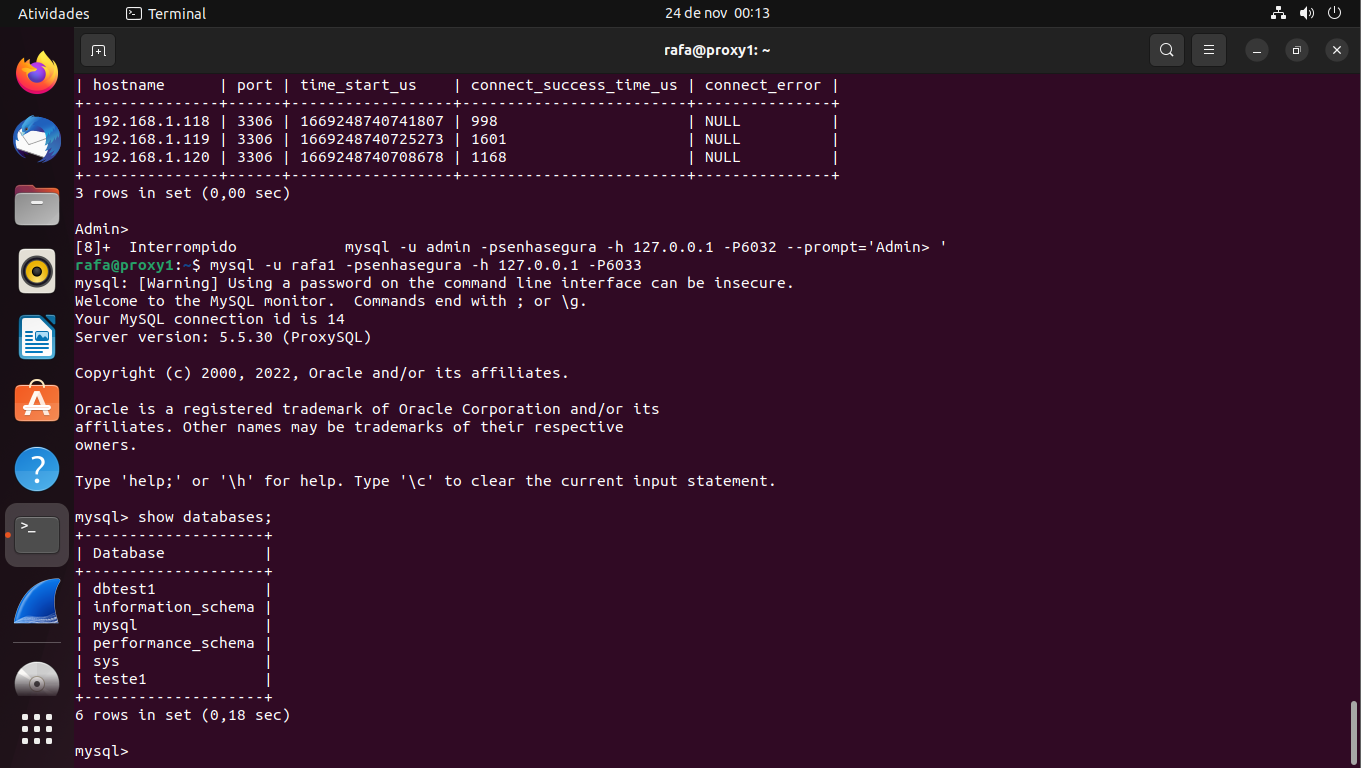
\includegraphics[width=13cm]{bd_proxy1.png}
\caption{Show Databases Proxy1}
\end{figure}

Concluída toda a configuração necessária do ProxySQL, estavam reunidas todas as condições para avançar com o Keepalived.

\newpage
\subsection{Instalação Keepalived}
A instalação do Keepalived foi feita nos dois proxies e para isso verificamos a seguinte instalação:

\begin{verbatim}apt-get install keepalived\end{verbatim}

\begin{figure}[H]
\center
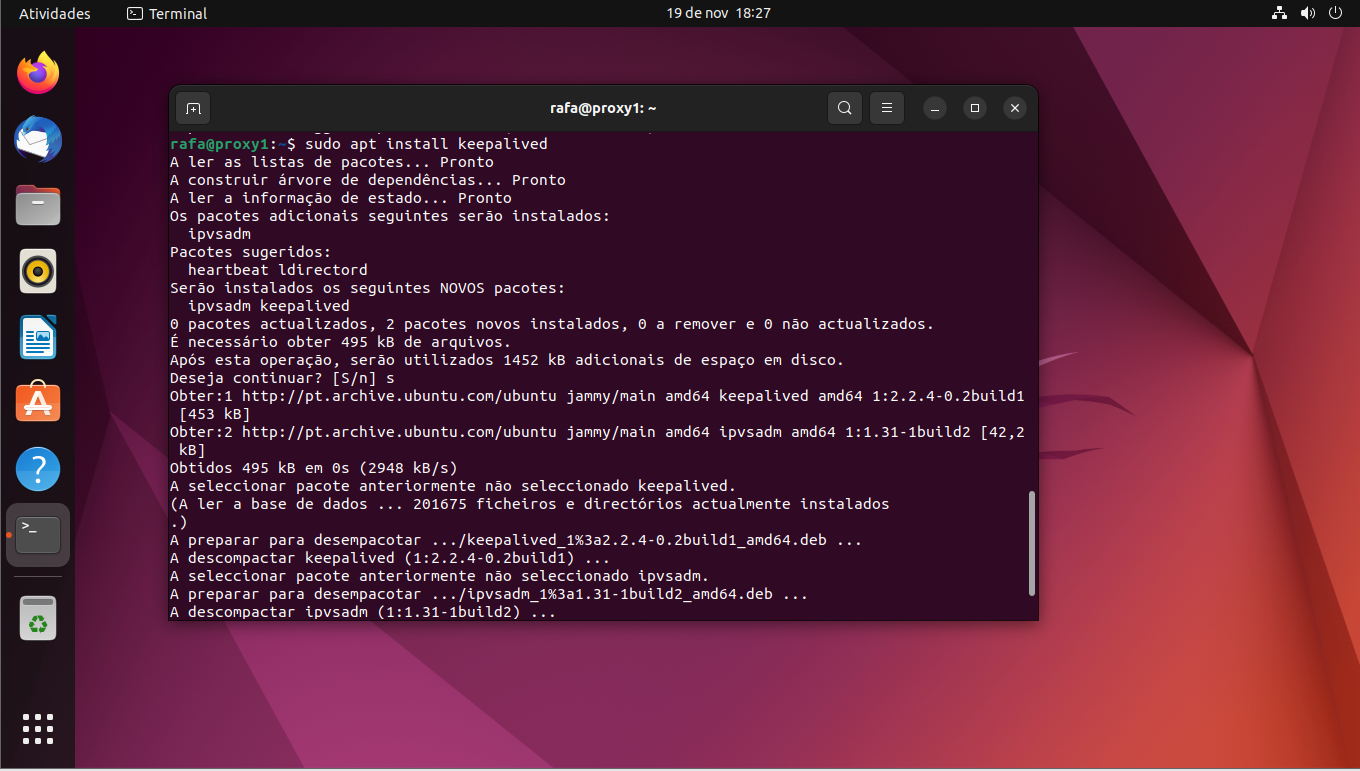
\includegraphics[width=13cm]{Screenshot_148.png}
\caption{Instalação Keepalived}
\end{figure}

\newpage
\subsection{Configuração Keepalived Proxy}
No ficheiro de configuração do Keepalived, \textit{/etc/keepalived/keepalived.conf}, vamos dar inicio á configuração com o intuito de verificar o \textit{MASTER} e \textit{BACKUP} entre os dois proxies.

\begin{verbatim}vrrp_instance V1_1{
        interface ens33
        state MASTER
        virtual_router_id 40
        priority 101
        authentication {
                auth_type PASS
                auth_pass senhasegura
        }       
        virtual_ipaddress {
                192.168.1.200/24
        }
}\end{verbatim}

\begin{figure}[H]
\center
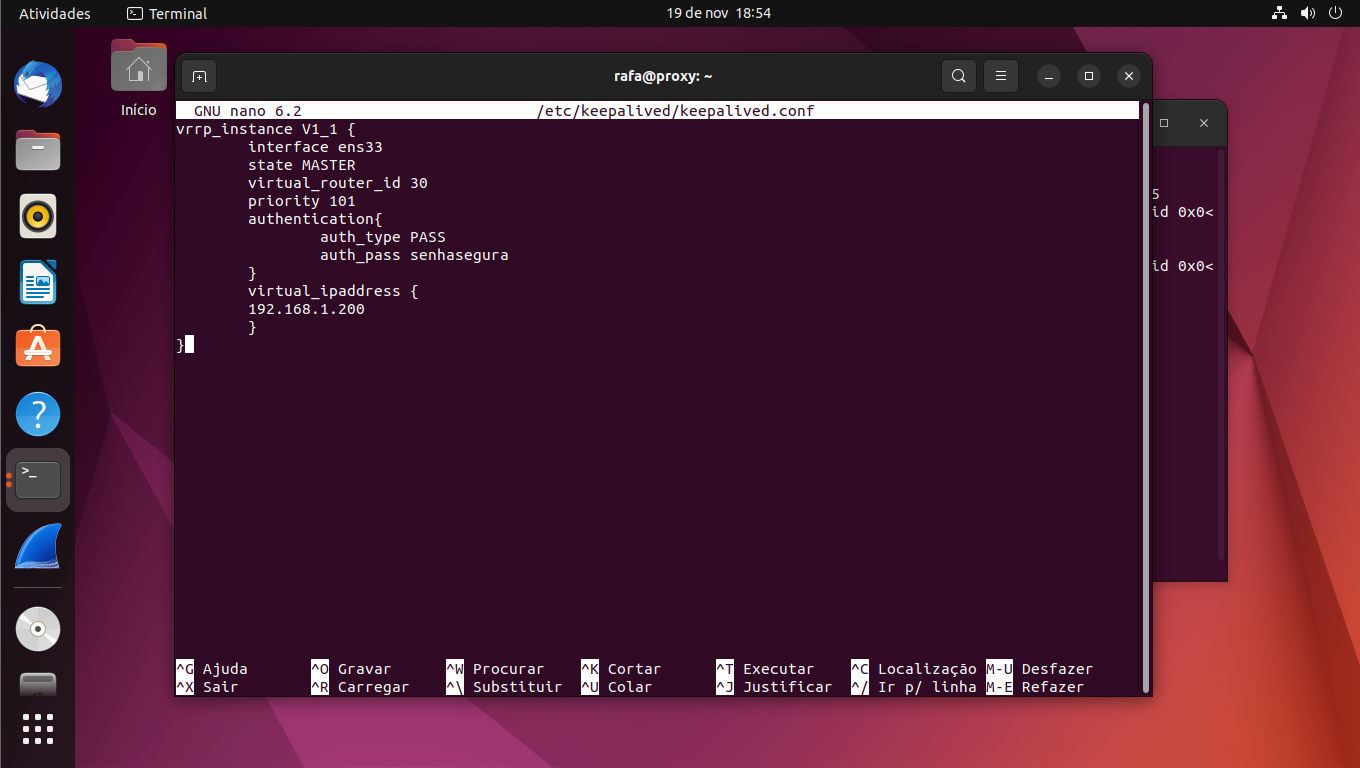
\includegraphics[width=13cm]{conf_master.png}
\caption{Keepalived Master Configuração}
\end{figure}

Depois da configuração convém reiniciar o serviço Keepalived:
\begin{verbatim}sudo service keepalived restart\end{verbatim}

\newpage
No Wireshark podemos verificar que já existe tráfego VRRP:
\begin{figure}[H]
\center
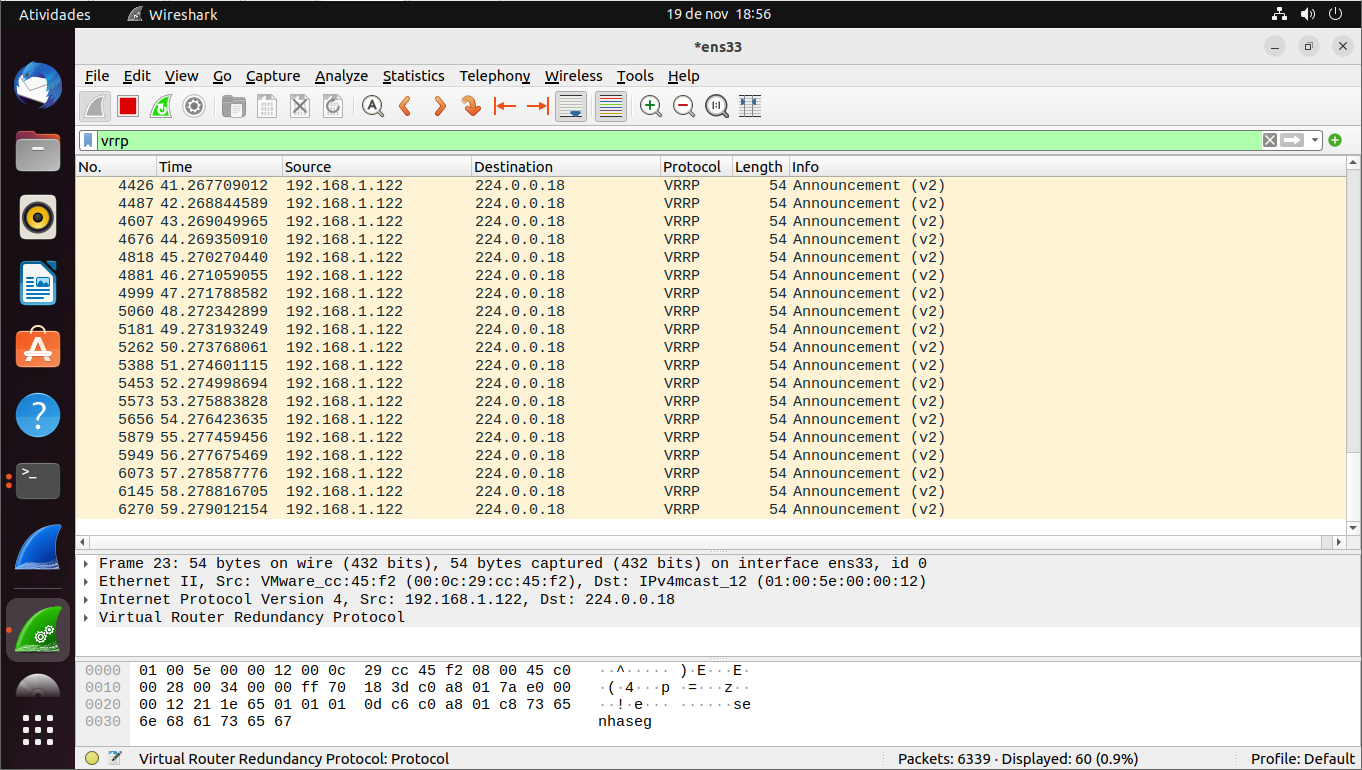
\includegraphics[width=13cm]{trafego_vrrp.png}
\caption{Tráfego VRRP}
\end{figure}

NOTA: Como o Keepalived de segundo a segundo envia um pacote e é MASTER, só verificamos tráfego do proxy, 192.168.1.122.

\hfill \break
\indent De seguida verificamos o \textit{status} do Keepalived:
\begin{verbatim}sudo service keepalived status\end{verbatim}

\begin{figure}[H]
\center
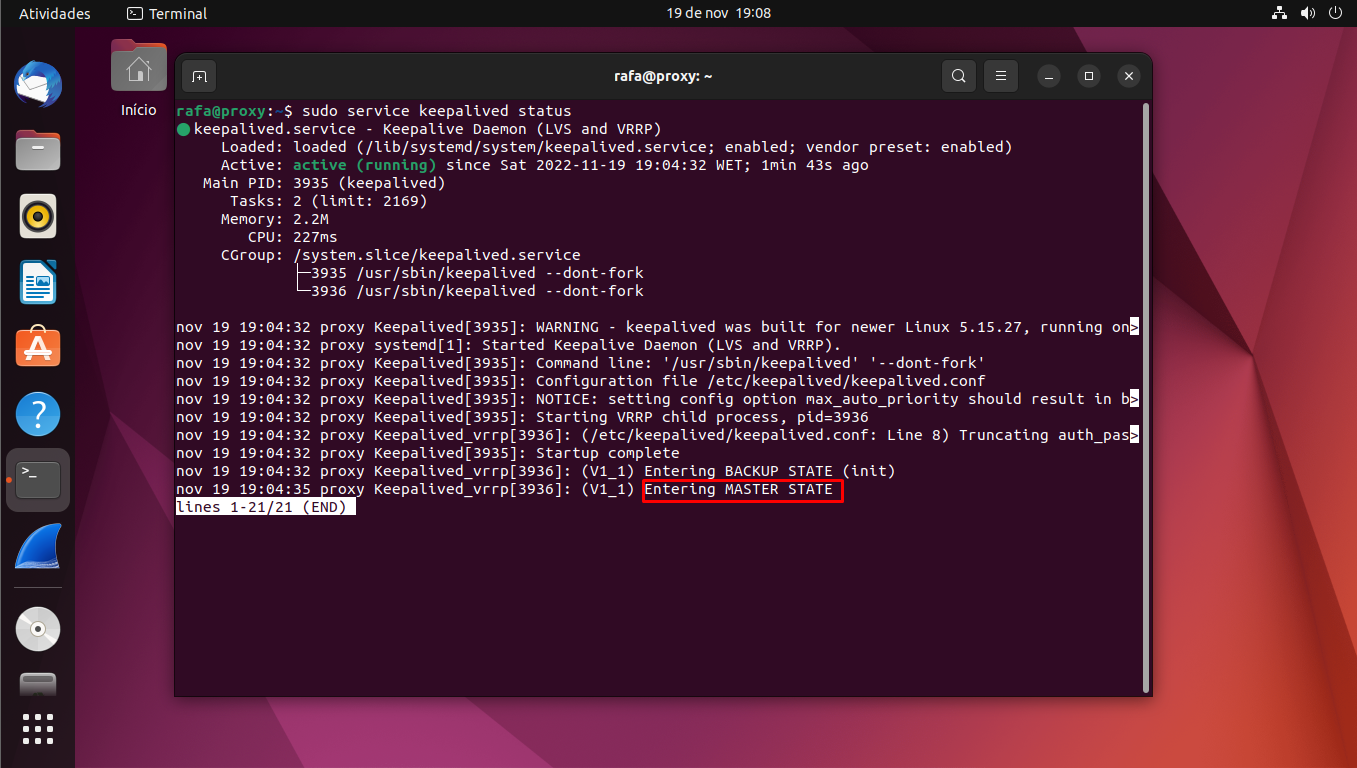
\includegraphics[width=13cm]{status_master.png}
\caption{Status Keepalived Master}
\end{figure}

Verificamos que o Proxy (192.168.1.122) é o MASTER.

\newpage
Ao verificar um pacote VRRP do Wireshark confirmei a prioridade do MASTER:

\begin{figure}[H]
\center
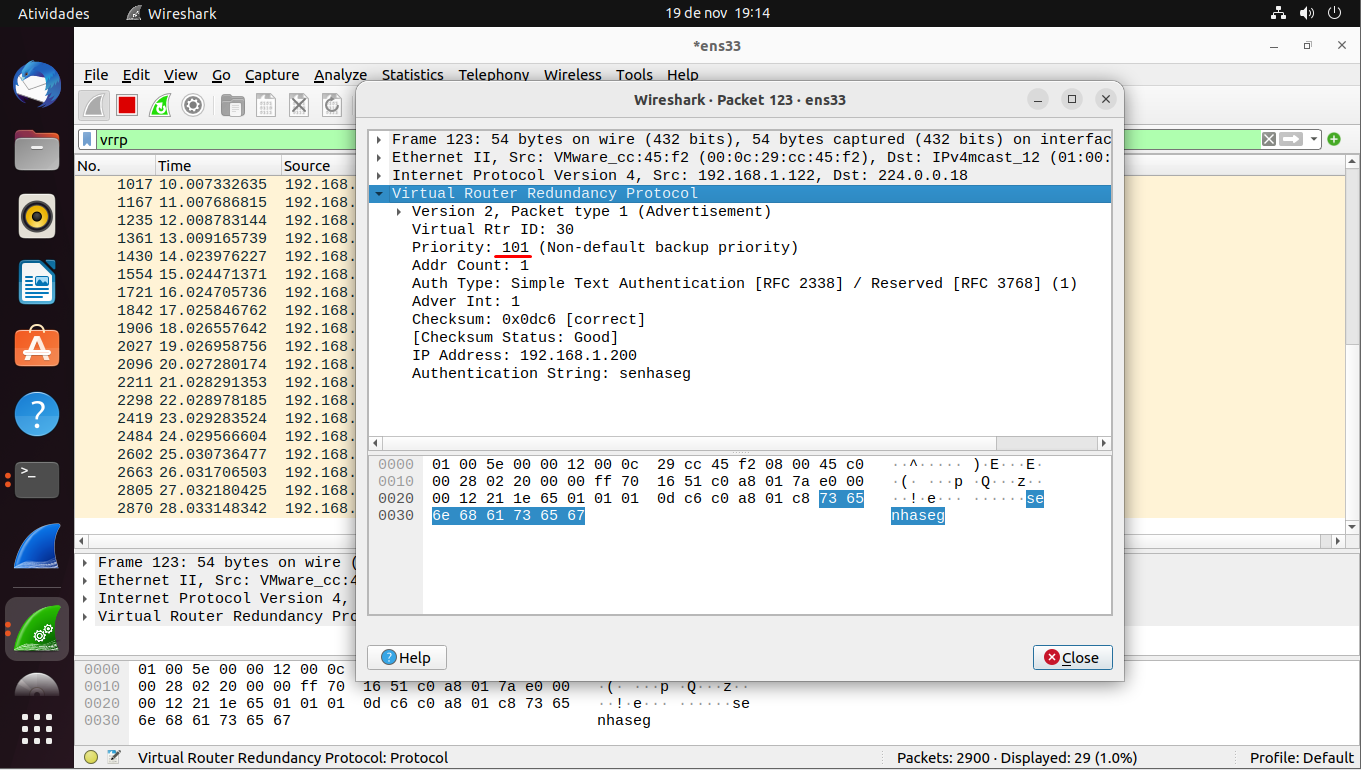
\includegraphics[width=13cm]{prioridade_master.png}
\caption{Prioridade Master}
\end{figure}


\newpage
\subsection{Configuração Keepalived Proxy1}
Repetindo o passo anterior da configuração do ficheiro do Keepalived:

\begin{verbatim}vrrp_instance V1_1{
        interface ens33
        state BACKUP
        virtual_router_id 40
        priority 100
        authentication {
                auth_type PASS
                auth_pass senhasegura
        }       
        virtual_ipaddress {
                192.168.1.200/24
        }
}\end{verbatim}

\begin{figure}[H]
\center
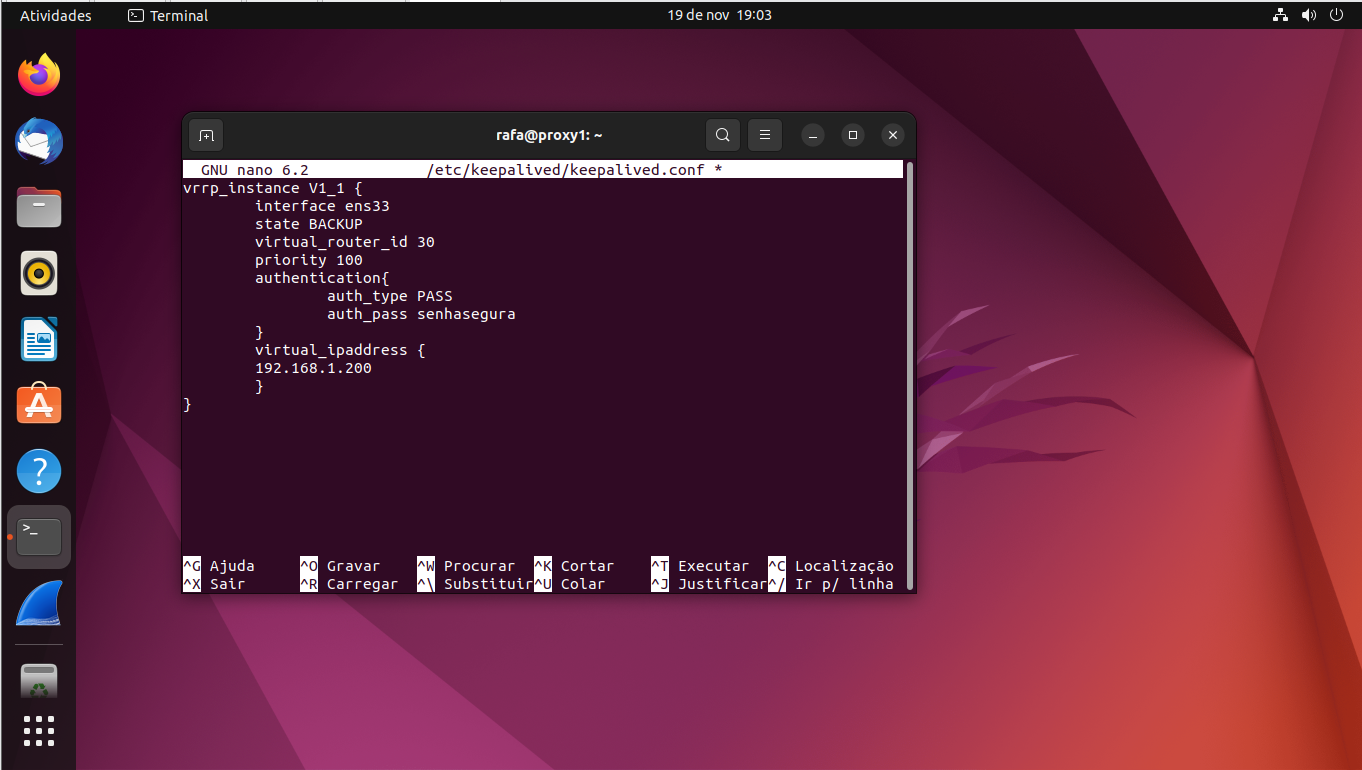
\includegraphics[width=13cm]{conf_back.png}
\caption{Keepalived Backup Configuração}
\end{figure}

Depois da configuração convém reiniciar o serviço Keepalived:
\begin{verbatim}sudo service keepalived restart\end{verbatim}

De seguida verificamos o \textit{status} do Keepalived:
\begin{verbatim}sudo service keepalived status\end{verbatim}

\begin{figure}[H]
\center
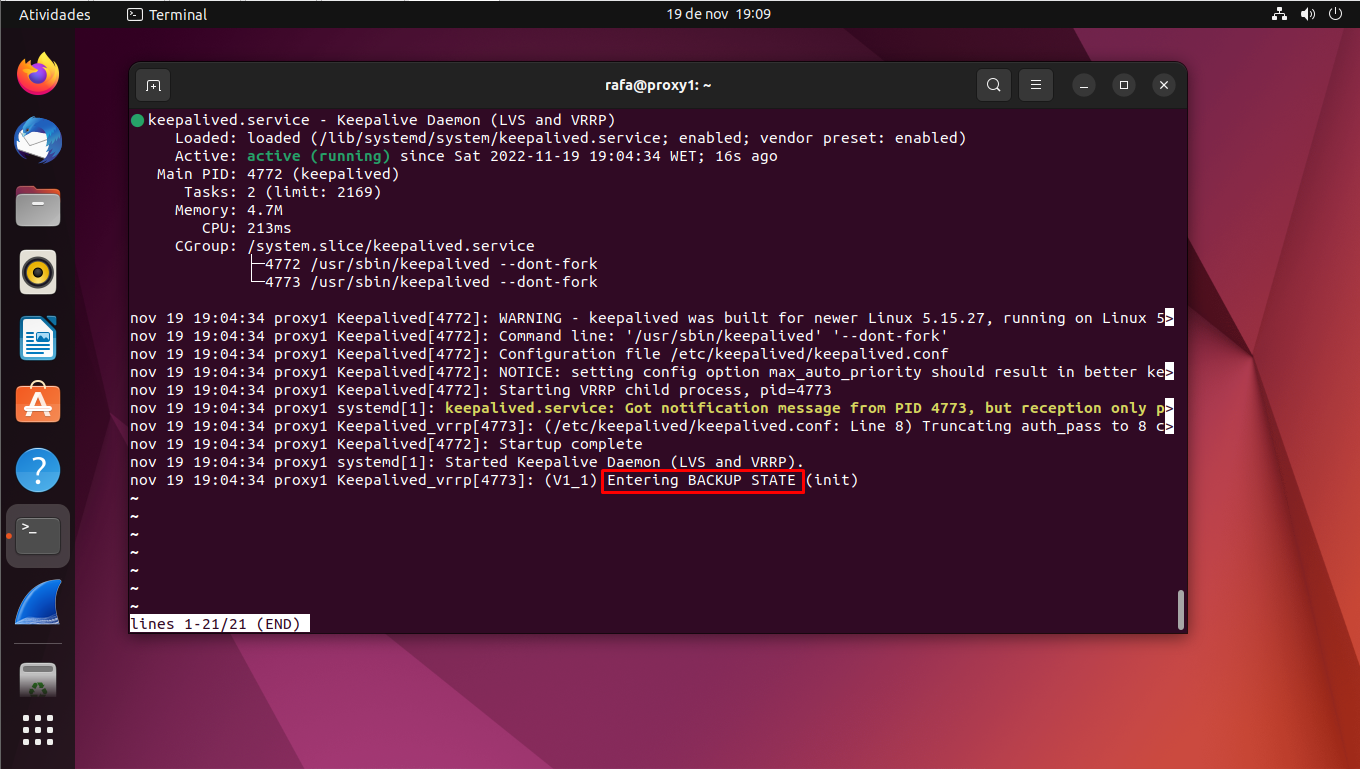
\includegraphics[width=13cm]{status_bak.png}
\caption{Status Keepalived Backup}
\end{figure}

Verificamos que o Proxy1 192.168.1.125 é o BACKUP.

\newpage
\section{Experiência}
O intuito desta experiência foi presenciar a troca de MASTER e BACKUP entre os dois proxies.  
\subsection{Estado atual dos proxies}
\begin{itemize}
    \item proxy (192.168.1.122): MASTER
    \item proxy1 (192.168.1.125): BACKUP
\end{itemize}

No proxy, ao desabilitar a interface \textit{ens33} com o comando \textit{ip link set ens3 down} verifiquei o STATUS, \textit{sudo service keepalived status}, do proxy1 e passou a ser MASTER.

\begin{figure}[H]
\center
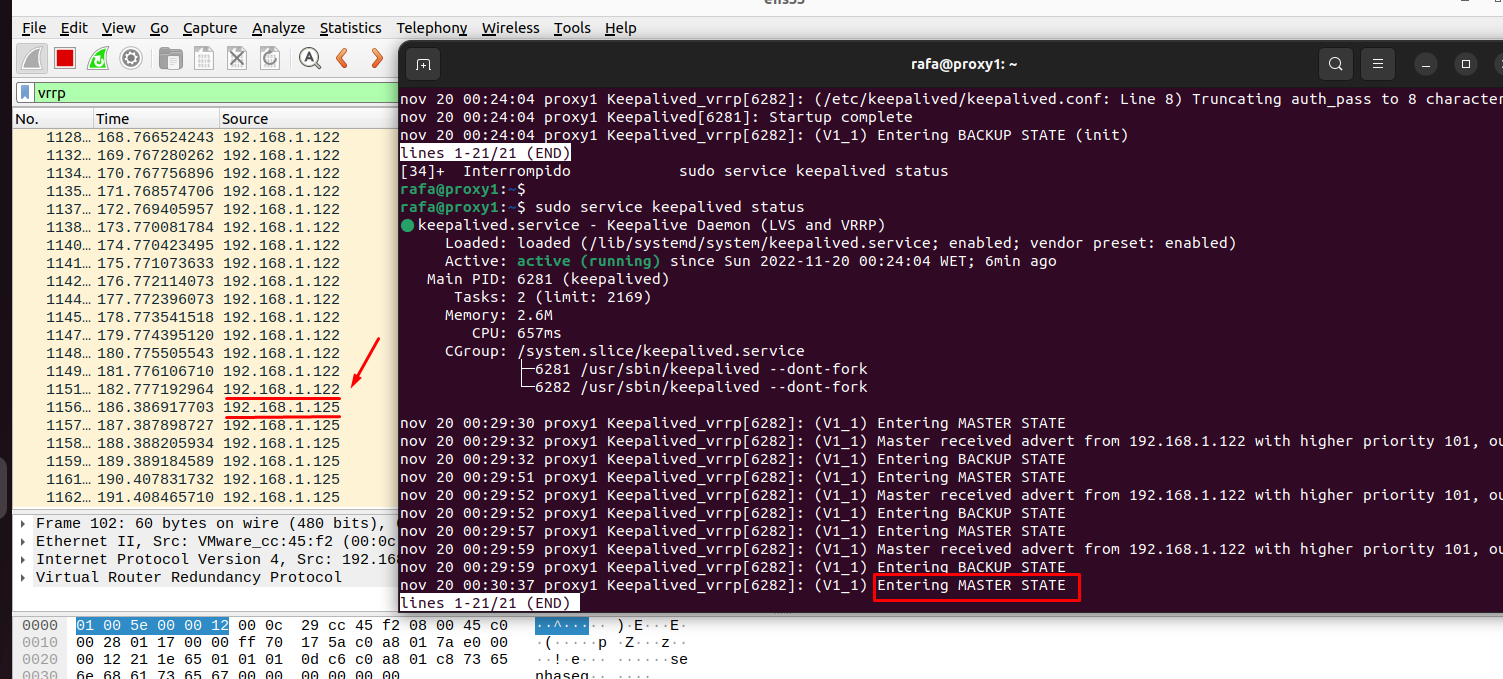
\includegraphics[width=13cm]{muda_status_proxy1.png}
\caption{Proxy1 Master}
\end{figure}

Ao mesmo tempo com o Wireshark a capturar tráfego verifiquei o momento em que o proxy 192.168.1.122 deixa de ser MASTER.

De seguida, ao habilitar a interface no proxy 192.168.1.122, \textit{ip link set ens3 up}, verificamos o seguinte:

\begin{figure}[H]
\center
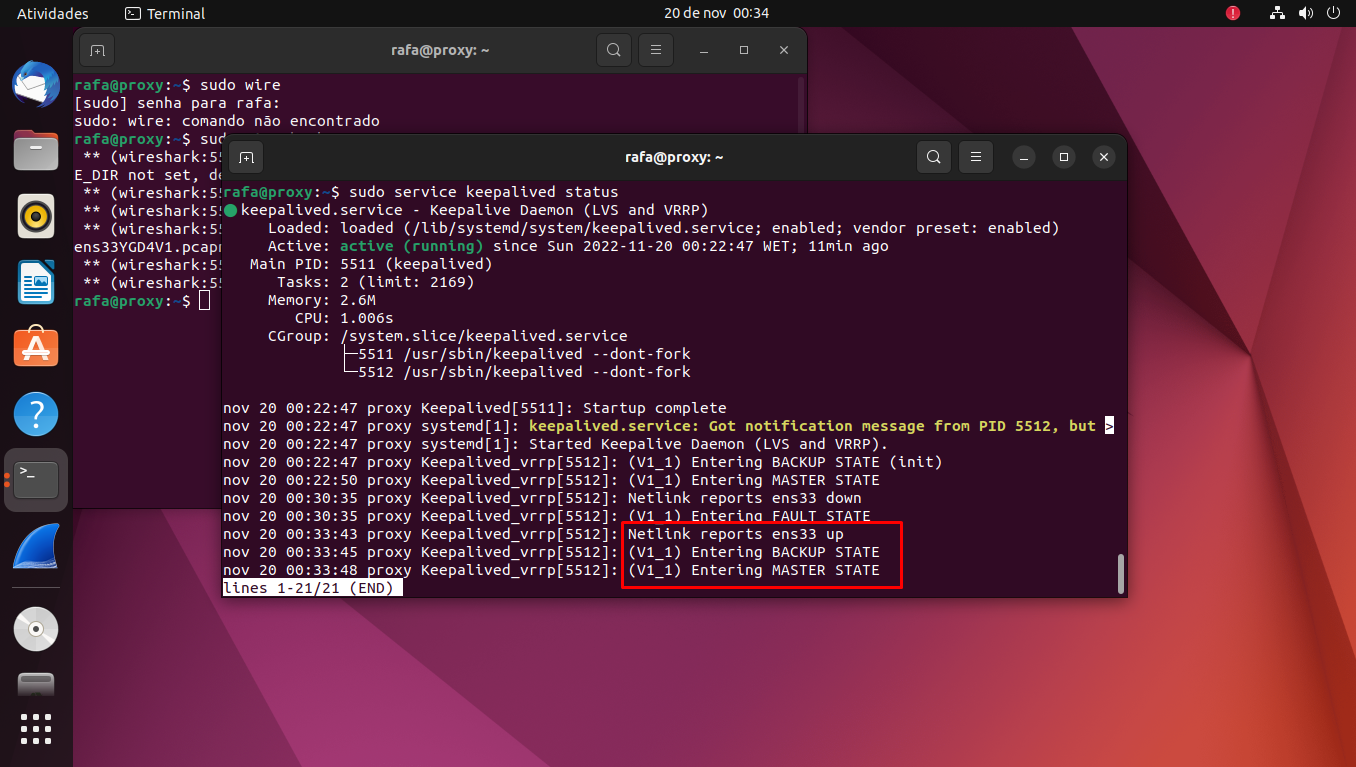
\includegraphics[width=13cm]{muda_status_proxy.png}
\caption{Proxy Master}
\end{figure}

\newpage
Verificou-se que, assim que a interface \textit{ens33} ficou \textit{up}, o proxy 192.168.1.122 voltou a MASTER por ter prioridade 101 e o proxy1 192.168.1.125 voltou a ser BACKUP.


\newpage
\section{Configuração DSR e Healthcheck Keepalived}
\subsection{Proxy}
Para a configuração do \ac{DSR} ou \textit{Direct Routing} e Healthcheck do Keepalived no proxy 192.168.1.122, foi feita a seguinte configuração:

\begin{verbatim}vrrp_instance V1_1{
    	interface ens33
    	state MASTER
    	virtual_router_id 40
    	priority 101
    	authentication {
        		auth_type PASS
        		auth_pass senhasegura
    	}	
    	virtual_ipaddress {
    		192.168.1.200/24 
    	}
}

virtual_server 192.168.1.200 6033 {
        delay_loop 10
        lb_algo rr
        lb_kind DR
        protocol TCP
    
        real_server 192.168.1.122 6033 {
            weight 1
            TCP_CHECK {
                  connect_timeout 10
                  connect_port    6033
            }
        }
        real_server 192.168.1.125 6033 {
            weight 1
            TCP_CHECK {
                  connect_timeout 10
                  connect_port    6033
            }
        }
}\end{verbatim}

Na configuração, o parâmetro \textit{weight} significa o peso relativo do servidor para fazer o balanceamento de carga. O \textit{lb\textunderscore  kind} seleciona um método de encaminhamento (NAT, DR, TUN). O \textit{lb\textunderscore algo} especifica o tipo de algoritmo utilizado para a disponibilidade, neste caso foi usado rr, \textit{Round-Robin}.


\newpage
Depois de guardar a configuração e dar \textit{restart} ao keepalived, \textit{sudo service keepalived restart}, verifiquei o \textit{status} do mesmo e verifiquei que o \textit{helthchecker} já estava ativado com o \textit{IP} Virtual:

\begin{figure}[H]
\center
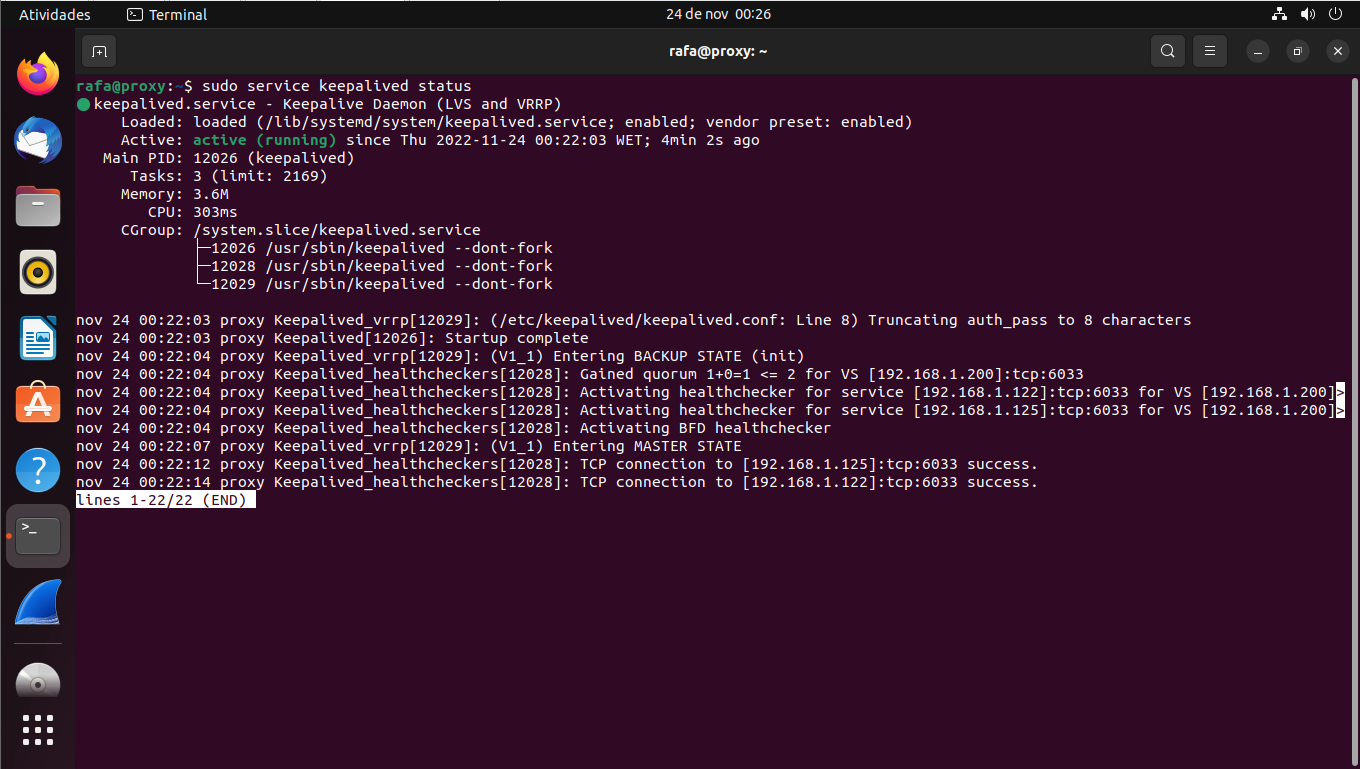
\includegraphics[width=13cm]{health_master.png}
\caption{DSR e Healthcheck Proxy}
\end{figure}

\subsection{Proxy1}
Para a configuração do \ac{DSR} ou \textit{Direct Routing} e Healthcheck do Keepalived no proxy1 192.168.1.125, foi feita a seguinte configuração:

\begin{verbatim}vrrp_instance V1_1{
    	interface ens33
    	state BAKCUP
    	virtual_router_id 40
    	priority 100
    	authentication {
        		auth_type PASS
        		auth_pass senhasegura
    	}	
    	virtual_ipaddress {
    		192.168.1.200/24 
    	}
}

virtual_server 192.168.1.200 6033 {
        delay_loop 10
        lb_algo rr
        lb_kind DR
        protocol TCP
    
        real_server 192.168.1.122 6033 {
            weight 1
            TCP_CHECK {
                  connect_timeout 10
                  connect_port    6033
            }
        }
        real_server 192.168.1.125 6033 {
            weight 1
            TCP_CHECK {
                  connect_timeout 10
                  connect_port    6033
            }
        }
}\end{verbatim}

\hfill \break
\indent De seguida guarda-se a configuração e faz-se o \textit{restart} ao keepalived, \textit{sudo service keepalived restart}, verifiquei novamente o mesmo acontecimento que foi mostrado na configuração do MASTER (proxy):

\begin{figure}[H]
\center
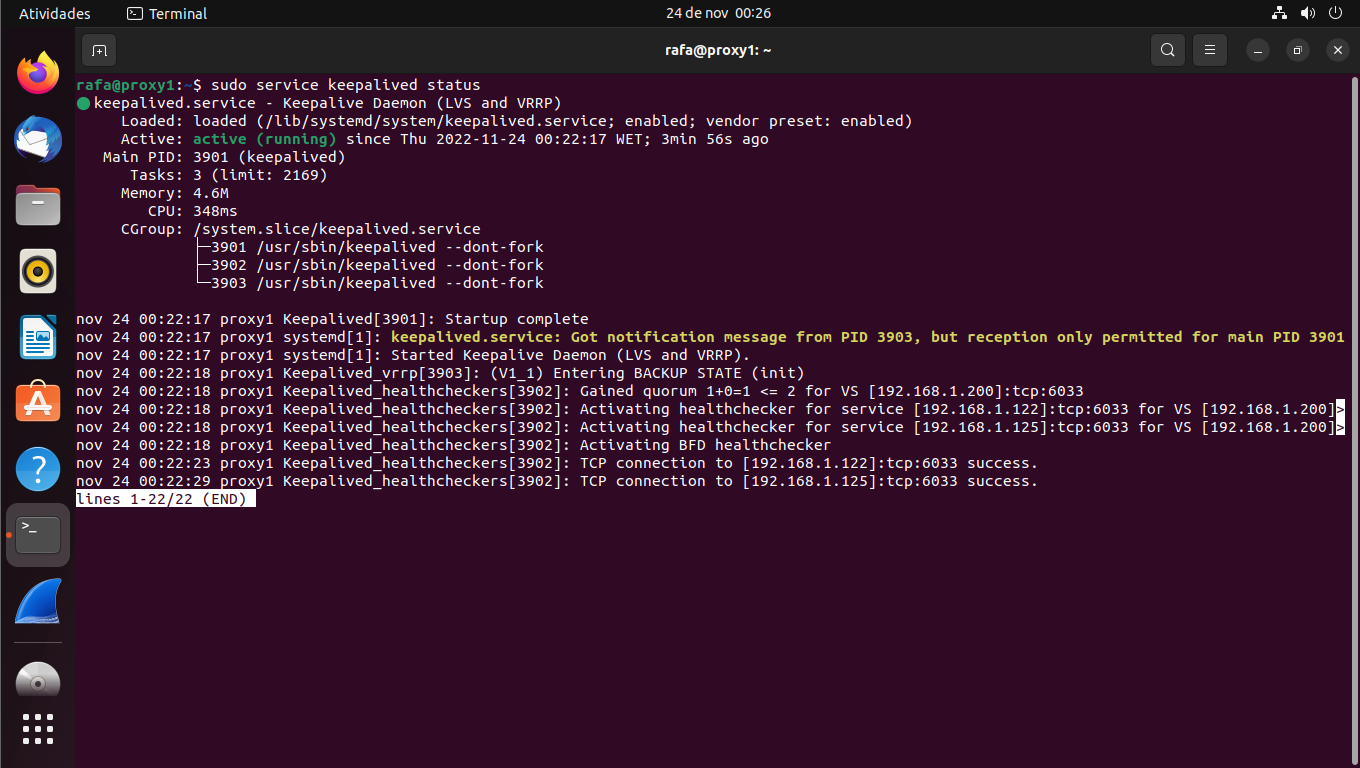
\includegraphics[width=13cm]{health_back.png}
\caption{DSR e Healthcheck Proxy1}
\end{figure}

Depois de verificar que o endereço \ac{IP} Virtual, 192.168.1.200, já se encontrava ativo verifiquei se estava associado á minha interface de rede:

\begin{verbatim}hostname -I\end{verbatim}

\begin{figure}[H]
\center
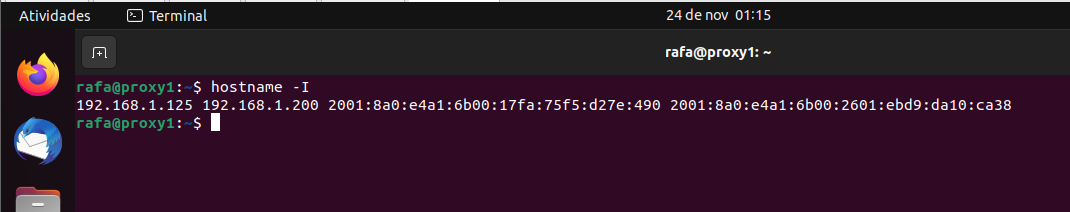
\includegraphics[width=13cm]{ipvirtual_proxy1.png}
\caption{IP Virtual}
\end{figure}

Verifica-se que o IP Virtual já se encontra associado á minha interface, assim como no proxy também se verifica.

\newpage
\section{Experiência}
Feita a configuração do Keepalived nos dois proxies tentei fazer a experiência de aceder à base de dados através do \ac{IP} Virtual. Para isso instalei o DBeaver no \ac{PC} Host.

Depois do DBeaver estar instalado criei uma conexão com a \ac{BD} MariaDB usando o \ac{IP} Virtual e o \ac{IP} do proxy 192.168.1.12:

\begin{figure}[H]
\center
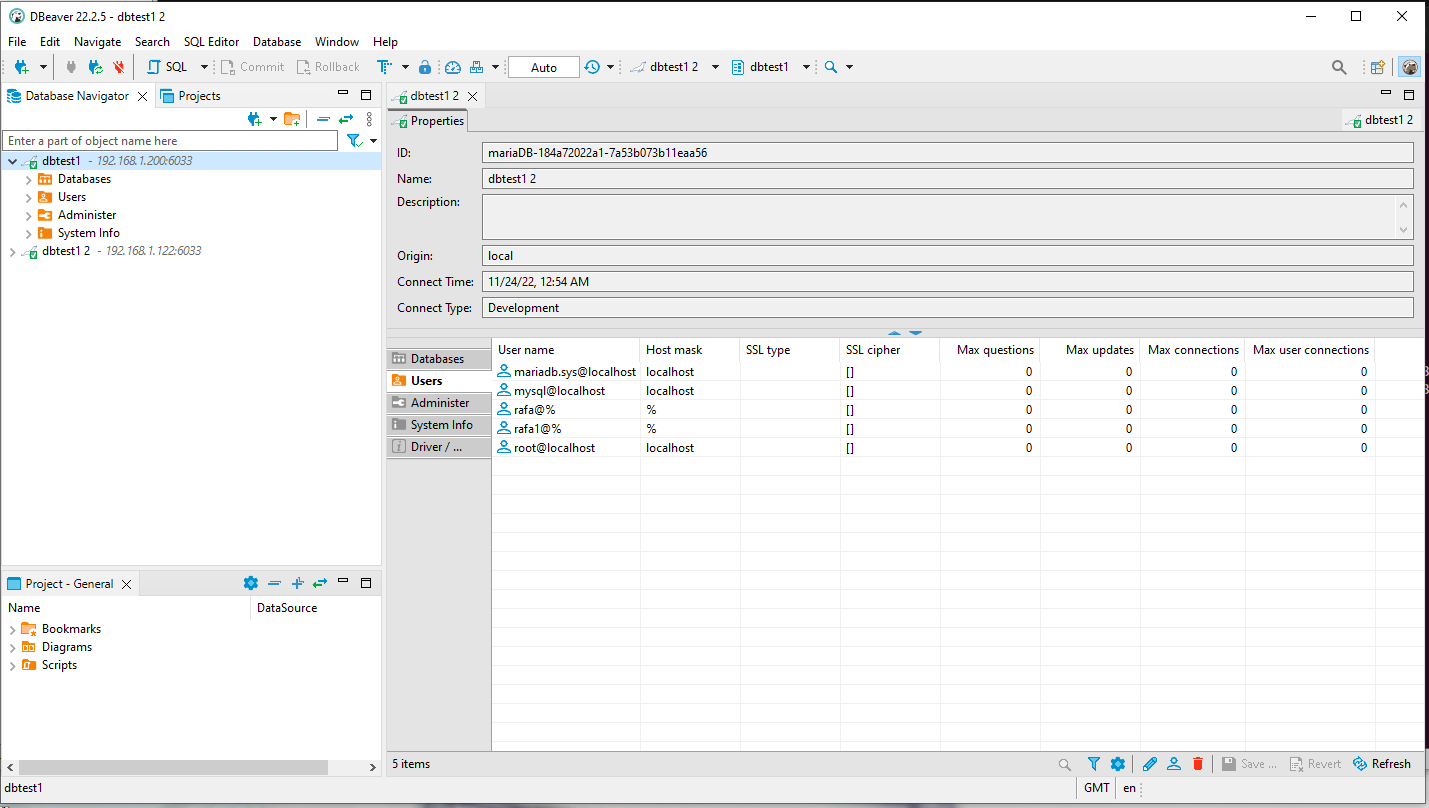
\includegraphics[width=13cm]{dbeaver.png}
\caption{DBeaver conexão}
\end{figure}

A conexão acima, com os dois proxies ligados, funcionou. Conseguia verificar as \ac{BD} existentes, os utilizadores MySQL que criei entre outras coisas.

\hfill \break
\indent Outra experiência que realizei foi aceder à \ac{BD} através do \ac{IP} Virtual mas com um proxy desligado. 
Para isso coloquei a \ac{VM} do proxy, 192.168.1.122. O proxy1, 192.168.1.125 entrou em modo \textit{MASTER} e consegui novamente no DBeaver aceder a \ac{BD} actravés do \ac{IP} Virtual, 192.168.1.200 com sucesso. 

Para esta última experiência não bastava desligar apenas o serviço Keepalived. Ao parar apenas o serviço Keepalived no proxy, 192.168.1.122, no DBeaver não conseguia estabelecer ligação à \ac{BD} com o \ac{IP} Virtual.

\begin{figure}[H]
\center
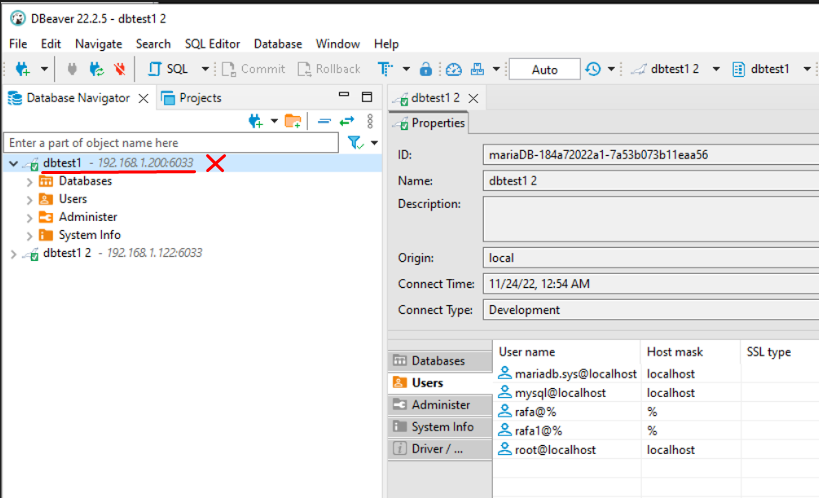
\includegraphics[width=13cm]{erro_dbeaver.png}
\caption{DBeaver Erro}
\end{figure}

Realizei várias experiências para compreender este problema e só consegui estabelecer ligação à \ac{BD} com o \ac{IP} Virtual colocando a \ac{VM} do proxy em \textit{pause} ou desligar.

